\documentclass{article}
\usepackage[preprint]{neurips_2025}
\usepackage[utf8]{inputenc}
\usepackage[T1]{fontenc}
\usepackage{hyperref}
\usepackage{url}
\usepackage{booktabs}
\usepackage{amsfonts,amsmath}
\usepackage{nicefrac}
\usepackage{microtype}
\usepackage{xcolor}
\usepackage{graphicx}
\usepackage{multirow}
\newcommand{\ttr}{t_{\mathrm{train}}}
\newcommand{\tva}{t_{\mathrm{val}}}

\title{Width Speeds Up Memorisation Faster Than Generalisation:\\
An Empirical Study of Delayed Generalisation on Modular Addition}

\author{Anonymous (autonomous-agent research run)}

\begin{document}
\maketitle

\begin{abstract}
Delayed generalisation (``grokking'') on modular arithmetic is mostly studied at one model size, so how it depends on scale is
poorly characterised. We state a falsifiable ``two-clock'' account---a memorisation clock that speeds up with width and a generalisation
clock governed by the weight-decay time scale---and register seven predictions before running the main sweeps.
We then test them with 434 full-batch AdamW runs (6 seeds per width in the core sweep; 2--6 elsewhere) on modular addition with
MLPs ($24$--$512$ hidden units), plus other operations, a modulus change, width-dependent learning-rate scalings and a small transformer.
In the core setting ($p{=}53$, 30\% of pairs for training), time to fit the training set falls as $w^{-1.0}$ to $w^{-1.4}$, whereas time to generalise
falls more slowly (log-log slope $-0.56$, 95\% CI $[-0.77,-0.36]$ for $w\ge128$), so the \emph{relative} delay $t_{val}/t_{train}$ grows with
width while the \emph{absolute} delay shrinks. The growth of the relative delay is not robust: it vanishes under a
$\mathrm{lr}\propto 1/w$ parameterisation that keeps the decay rate $\mathrm{lr}\cdot\mathrm{wd}$ fixed, reverses
(wider models generalise later) when the decay rate falls with width, and is absent for $p{=}97$ and for some operations.
Memorisation time is indistinguishable between true and random labels (Spearman $\rho{=}0.9999$ over 28 width--data-fraction cells), and
fitting requires only $\approx$4--5 parameters per training example, but generalising needs several times more width: narrow models that fit the
training set stay at chance for $10^5$ steps and generalise only after $2$--$3\times10^5$ steps, so the ``threshold'' is a budget-dependent
soft boundary. Of the seven registered predictions, three are supported, three are partly supported (one component falsified in each) and one is falsified: at fixed width, generalisation time does not depend on learning rate and weight decay only through their product;
a post-hoc test shows that a product-like dependence emerges only at large width. Scope limits: one small modulus, one optimiser recipe, $\le 6$ seeds, and the transformer evidence is weak.
\end{abstract}

\section{Introduction}
Neural networks trained on small algorithmic datasets can reach perfect training accuracy long before validation accuracy rises~\citep{power2022grokking}.
Explanations include mechanistic circuit formation~\citep{nanda2023progress}, a loss-landscape/weight-norm picture~\citep{liu2023omnigrok},
efficiency of competing circuits under weight decay~\citep{varma2023circuit}, and a lazy-to-rich transition of the training dynamics~\citep{kumar2024grokking}.
Most such studies fix the architecture size. Yet experimenters routinely choose the width of the model when building grokking testbeds,
and the choice can change both \emph{whether} and \emph{how strongly} delayed generalisation appears. We ask:
\emph{on modular arithmetic, how does the occurrence of delayed generalisation depend on model scale?}

Rather than just plotting delay against size, we put forward an explanation that makes checkable predictions, state the predictions before the main
experiments, and report which are falsified. The explanation (Sec.~\ref{sec:hyp}) says that two ``clocks'' scale differently with width:
fitting the training labels (memorisation) speeds up quickly with width, while generalisation is released on a time scale set by weight decay.
Our contributions are empirical:
\begin{itemize}\setlength\itemsep{0pt}
\item A measurement protocol with bootstrap uncertainty and explicit handling of censored runs (as lower bounds), and a self-registered predictions file written before the main sweeps (\texttt{code/PREREG.md}).
\item In the core setting, the memorisation clock scales as $w^{-1.0}\!\ldots w^{-1.4}$ and is label-agnostic, whereas the generalisation clock
scales much more weakly at large width (steeply near a threshold), so relative delay grows and absolute delay shrinks with width (Sec.~\ref{sec:core},\ref{sec:mem}).
\item Fitting and generalising have very different capacity thresholds, and the latter is a soft, budget-dependent boundary; with more data, narrow models generalise without any delay (Sec.~\ref{sec:thresh}).
\item The width--delay relation is \emph{parameterisation dependent}: depending on how lr and wd scale with width, relative delay grows, stays flat, or grows faster, and absolute generalisation time can even increase with width (Sec.~\ref{sec:timescale},\ref{sec:robust}).
\item An honest scorecard (Table~\ref{tab:score}): of seven registered predictions, 3 are supported (P1, P2 in the core setting, P7), 3 are partly supported (P3, P5, P6) and 1 is falsified (P4).
\end{itemize}

\section{Related work}
\textbf{Grokking.} \citet{power2022grokking} introduced delayed generalisation on algorithmic datasets, including modular arithmetic.
\citet{nanda2023progress} reverse-engineer a one-layer transformer on modular addition and define progress measures; \citet{liu2023omnigrok} relate grokking to weight norm and
initialisation scale and extend it beyond algorithmic data; \citet{varma2023circuit} explain it via the relative efficiency of memorising and generalising circuits and
test predictions by training experiments; \citet{kumar2024grokking} connect it to a lazy-to-rich dynamics transition in two-layer networks.
\citet{davies2023unifying} discuss grokking together with double descent~\citep{nakkiran2020deep}. We do not test any of these mechanisms directly
(we do no interpretability); we use them to motivate predictions on how timing should scale with width, learning rate and weight decay.\\
\textbf{Memorisation capacity.} \citet{zhang2017rethinking} show that networks fit random labels; \citet{tirumala2022memorization} and \citet{morris2025memorize}
study memorisation in language models, the latter with a method that estimates how much information a model holds about its data points. Our random-label probe is a small-scale analogue used to time
the ``memorisation clock''. \\
\textbf{Optimiser.} We use AdamW~\citep{loshchilov2017decoupled}, in which weight decay shrinks weights by a factor $(1-\mathrm{lr}\cdot\mathrm{wd})$ per step, which is why the product $\mathrm{lr}\cdot\mathrm{wd}$ appears in our time-scale prediction.\\
\textbf{Positioning.} Prior work (e.g.\ \citealp{power2022grokking,liu2023omnigrok}) varies data fraction, weight decay and initialisation scale; here we focus on \emph{model width as the controlled variable}, separate absolute from relative delay, and
stress-test conclusions against optimiser parameterisation and censoring.

\section{Setup, hypothesis and registered predictions}\label{sec:setup}
\textbf{Data.} For a prime $p$ and operation $\circ$, all $p^2$ pairs $(a,b)$ are enumerated with label $a\circ b \bmod p$
(add, sub, mul, or $a^2{+}b^2$); a random fraction $f$ (default $0.3$) is the training set and the rest the validation set. Main modulus: $p{=}53$ ($843$ training pairs);
$p{=}97$ is a robustness check. Data are generated in memory (no download).\\
\textbf{Models.} (i) MLP: learned $w$-dim embeddings of $a$ and $b$, concatenated, two hidden ReLU layers of width $w$, linear readout to $p$ logits ($4$k--$842$k parameters for $w{=}24$--$512$).
(ii) One-layer transformer ($d_{model}{=}w$, 4 heads, MLP $4w$, no LayerNorm; input tokens $[a,b,=]$). Initialisation: all weight matrices $\mathcal N(0,1/\text{fan-in})$ (He scale for MLP hidden layers), i.e.\ a standard (``SP'') parameterisation.\\
\textbf{Training.} Full-batch AdamW ($\beta{=}(0.9,0.98)$, lr $10^{-3}$, wd $1.0$, 10-step warm-up), cross-entropy, up to $T_{max}$ steps ($10^5$ for most MLP runs). Accuracy is evaluated every 10 steps up to step 500, every 50 up to 5000, then every 200.
Each \emph{seed} controls the initialisation and the train/validation split.\\
\textbf{Metrics.} $\ttr$ ($\tva$): first evaluation step with train (validation) accuracy $\ge0.99$. Relative delay $R=\tva/\ttr$, absolute delay $D=\tva-\ttr$.
Runs that do not reach the threshold by $T_{max}$ are \emph{censored} and their value is set to $T_{max}$ (a lower bound); medians over seeds are therefore bounds when $\ge$ half of the runs are censored (hollow markers, ``$\ge$'' in tables).
Uncertainty: 95\% bootstrap CI of the median (4000 resamples of seeds); log-log slopes are fit to per-width medians, with CIs from bootstrap resampling of seeds within width.
$\ttr$ has a resolution of 10 steps for $\ttr\le500$ (e.g.\ $\pm25\%$ at $\ttr{=}20$), which bootstrap CIs do not capture.
Slopes and rank correlations use only widths where fewer than half of the runs are censored unless stated.

\subsection{Explanation under test: a ``two-clock'' account}\label{sec:hyp}
\emph{Memorisation clock} $t_{mem}(w)$: how fast the network fits training labels; it is limited by memorisation speed and should shorten quickly with width.
\emph{Generalisation clock} $t_{gen}$: when weight decay has pruned the memorising solution enough for the generalising circuit to take over; it should be set mainly by the optimiser time scale $1/(\mathrm{lr}\cdot\mathrm{wd})$ and depend only weakly on width.
Registered predictions (full text with falsification criteria in \texttt{code/PREREG.md}; written after an exploratory pilot, seeds 0--2, but before the sweeps with seeds 100+):
\begin{description}\setlength\itemsep{0pt}
\item[P1] $\ttr$ decreases monotonically with width (negative log-log slope).
\item[P2] $R$ increases with width while $D$ does not increase.
\item[P3] Random-label fitting time tracks real-label $\ttr$ (Spearman $>0.8$), and the smallest width that fits random labels predicts the smallest width that fits true labels within a factor 1.5, shifting to larger widths with more training data.
\item[P4] At fixed width, $\tva$ depends on lr and wd through lr$\cdot$wd: log-log slope in $[-1.3,-0.7]$, and equal-product pairs differ by $<1.5\times$.
\item[P5] P1 and P2 hold for sub, mul, $a^2{+}b^2$ and $p{=}97$.
\item[P6] P1, P2 hold for the transformer.
\item[P7] (exploratory) The width trend changes if lr is scaled with width, i.e.\ it depends on the parameterisation.
\end{description}
A post-hoc, clearly exploratory prediction P8 (Sec.~\ref{sec:timescale}) was registered after the main sweeps and before its test.

\section{Experiments and results}
All experiments use the code in \texttt{code/}; Appendix~\ref{app:exp} lists which script and result file produce each figure and table.
Counts of runs per cell are given in tables; because $n\le6$ seeds per cell, CIs are coarse and we avoid claims resting on small differences.
No multiple-comparison correction was applied: we report effect sizes with CIs rather than p-values, and no conclusion rests on a single borderline test.

\subsection{Core sweep: scale makes the delay relatively longer but absolutely shorter}\label{sec:core}
\begin{figure}[t]
\centering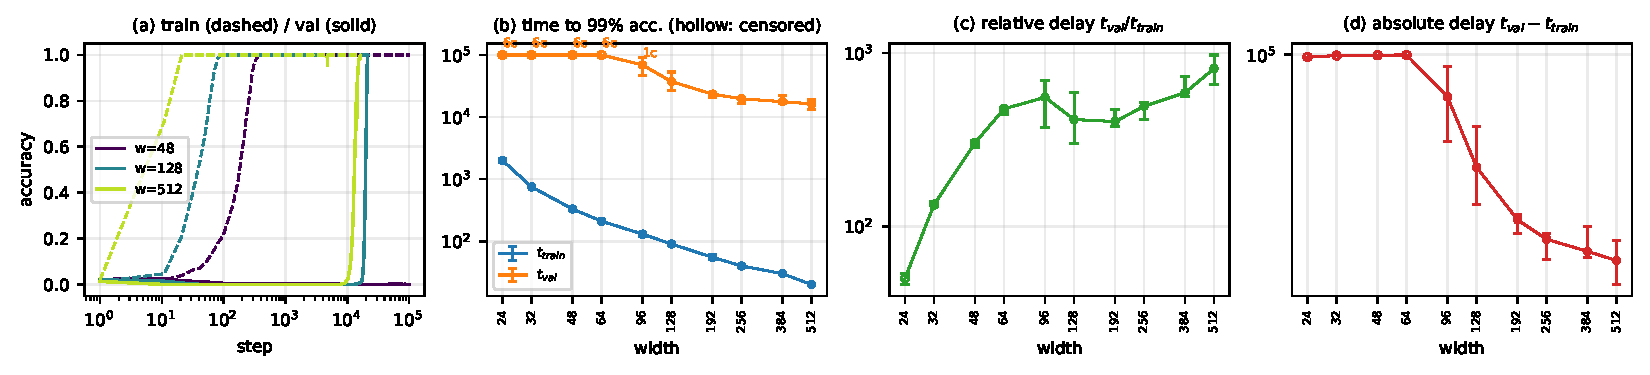
\includegraphics[width=\linewidth]{figs/fig_e1.pdf}
\caption{Core MLP width sweep (modular addition, $p{=}53$, $f{=}0.3$, 6 seeds/width). (a) Example runs (seed 100). (b) Time to 99\% accuracy; median and bootstrap 95\% CI;
hollow markers: $\ge$ half the runs censored at $10^5$ steps. (c) Relative delay $R$. (d) Absolute delay $D$.}\label{fig:e1}
\end{figure}
\begin{table}[t]\centering\scriptsize
\caption{Core sweep. Median [95\% bootstrap CI] over 6 seeds; steps. cens.: runs not reaching 99\% validation accuracy within $10^5$ steps. For widths $\le64$, $t_{val}$, $R$, $D$ are lower bounds (censored).}\label{tab:e1}
\begin{tabular}{rrcccccc}
\toprule
width & params & $t_{train}$ & $t_{val}$ & $R$ & $D$ & cens. & $n$ \\
\midrule
24 & 4k & 2000 [1875,2175] & $\geq$100000 [100000,100000] & $\geq$50 [46,53] & $\geq$98000 [97825,98125] & 6/6 & 6 \\
32 & 7k & 750 [725,750] & $\geq$100000 [100000,100000] & $\geq$133 [133,138] & $\geq$99250 [99250,99275] & 6/6 & 6 \\
48 & 12k & 330 [320,350] & $\geq$100000 [100000,100000] & $\geq$303 [286,312] & $\geq$99670 [99650,99680] & 6/6 & 6 \\
64 & 19k & 210 [210,225] & $\geq$100000 [100000,100000] & $\geq$476 [445,476] & $\geq$99790 [99775,99790] & 6/6 & 6 \\
96 & 38k & 130 [120,130] & 69100 [46700,90400] & 555 [373,695] & 68975 [46575,90270] & 1/6 & 6 \\
128 & 63k & 90 [90,90] & 37200 [26900,53200] & 413 [299,591] & 37110 [26810,53110] & 0/6 & 6 \\
192 & 131k & 55 [50,60] & 23400 [20800,24400] & 402 [378,474] & 23345 [20745,24345] & 0/6 & 6 \\
256 & 224k & 40 [40,40] & 19700 [16500,20700] & 492 [412,518] & 19660 [16460,20660] & 0/6 & 6 \\
384 & 484k & 30 [30,30] & 17700 [16800,22000] & 590 [560,733] & 17670 [16770,21970] & 0/6 & 6 \\
512 & 842k & 20 [20,20] & 16300 [13200,19500] & 815 [660,975] & 16280 [13180,19480] & 0/6 & 6 \\
\bottomrule
\end{tabular}
\end{table}
Figure~\ref{fig:e1} and Table~\ref{tab:e1} show the core sweep. Training accuracy reaches 99\% in $\ttr=2000$ steps at $w{=}24$ and $20$ steps at $w{=}512$.
Over the ten widths the log-log slope of $\ttr$ is $-1.39$ [$-1.40,-1.37$]; restricted to $w\ge128$ it is $-1.04$ [$-1.06,-1.02$] (Spearman $\rho=-0.997$ over 30 runs): \textbf{P1 is supported}.
Validation accuracy tells a different story. For $w\le64$ none of 24 runs reaches 99\% validation accuracy in $10^5$ steps (final validation accuracy $\le 0.07$, i.e.\ near chance $1/53$), at $w{=}96$ five of six runs do, and for $w\ge128$ all do.
Among $w\ge128$, $\tva$ falls from $37.2$k to $16.3$k steps: slope $-0.56$ [$-0.77,-0.36$] (Spearman $\rho=-0.81$ [$-0.92,-0.60$]), i.e.\ shallower than $\ttr$ (slope difference $\approx0.5$).
Consequently $R$ rises from $413$ ($w{=}128$) to $815$ ($w{=}512$) (slope $+0.49$ [$+0.25,+0.71$]; $\rho=+0.78$ [$0.51,0.94$]), while $D$ falls from $37$k to $16$k (slope $-0.56$ [$-0.77,-0.34$]): \textbf{P2 is supported for this setting}.
$R$ is not monotone in $w$ at intermediate widths ($555,413,402,492,590,815$ for $w{=}96\ldots512$), so the claim is about the trend.
The local slope of $\tva$ is much steeper at small width ($-2.2$ for $96\to128$, $-1.1$ for $128\to192$, $-0.6$ for $192\to256$) than at large width ($-0.26$ for $256\to384$, $-0.29$ for $384\to512$): $\tva$ appears to
flatten towards a floor of roughly $1.5\times10^4$ steps, about $15/(\mathrm{lr}\cdot\mathrm{wd})$. The final parameter $L_2$ norm is $41$--$48$ for all widths $\ge24$, whether the model memorised or generalised, so this norm does not distinguish the two phases here.

\subsection{The memorisation clock is label-agnostic}\label{sec:mem}
\begin{figure}[t]
\centering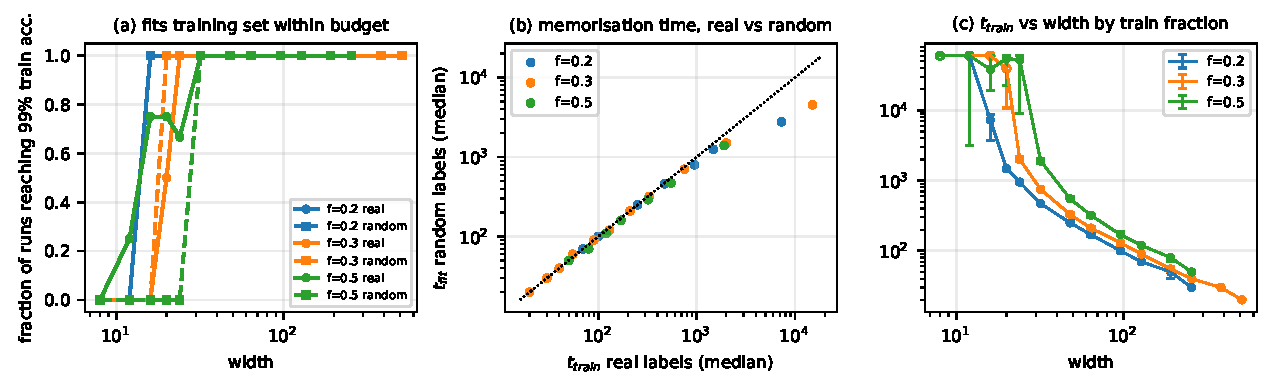
\includegraphics[width=\linewidth]{figs/fig_probe.pdf}
\caption{Memorisation probe (MLP, $p{=}53$, three training fractions $f$; random-label runs use the same training inputs with uniformly random labels). (a) Fraction of runs reaching 99\% train accuracy within budget (60--100k steps; 3--6 seeds). (b) Median fitting time, random vs.\ real labels, one point per (width, $f$) cell where both fit. (c) $\ttr$ vs width, real labels (hollow: censored).}\label{fig:probe}
\end{figure}
We repeat training on random labels (same inputs, 3 seeds per cell, 28 (width,$f$) cells where both label types fit). Median fitting times for random and true labels are almost identical
(Fig.~\ref{fig:probe}b; Spearman $\rho=0.9999$ [$0.998,1.0$] on log scale, median ratio $0.96$): the time to fit is a property of the model and training-set size rather than of label structure, supporting
the interpretation of $\ttr$ as a memorisation clock (first half of \textbf{P3 supported}).
With random labels the smallest width at which at least half of runs fit is $16$, $20$, $32$ for $f{=}0.2,0.3,0.5$, i.e.\ $2.5$k, $3.4$k, $6.5$k parameters for $562$, $843$, $1404$ training pairs:
$\approx4.4$, $4.0$, $4.6$ parameters per training example (wd$=1$, budget $\le 10^5$ steps). So capacity needed for \emph{fitting} grows roughly proportionally to the amount of data.
The second half of P3 is \textbf{falsified at $f{=}0.5$}: true labels are fitted from $w{=}16$ (3/4 runs) while random labels need $w{=}32$ (a factor 2 $>1.5$), because small models can fit true labels by learning the rule
(Sec.~\ref{sec:thresh}). At $f{=}0.2$ and $0.3$ the thresholds agree ($16$ vs $16$; $20$ vs $20$), and thresholds shift to larger width with more data as predicted (random labels).

\subsection{Fitting is cheap; generalising needs far more width, and the boundary is soft}\label{sec:thresh}
\begin{figure}[t]
\centering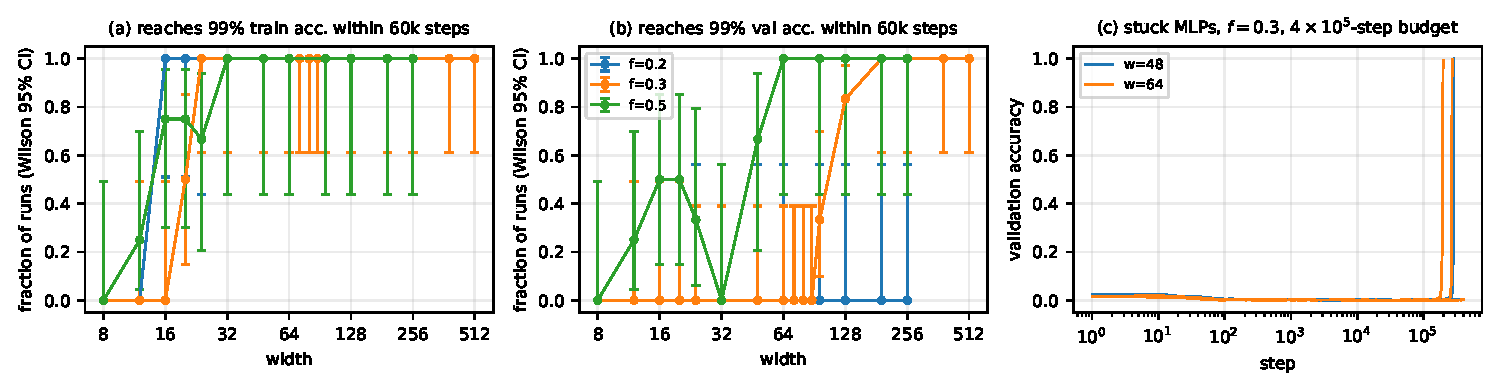
\includegraphics[width=\linewidth]{figs/fig_thresh.pdf}
\caption{(a,b) Fraction of runs reaching 99\% train / validation accuracy within 60k steps vs width, for three training fractions (3--6 seeds per cell; Wilson 95\% CIs). (c) Validation accuracy of narrow MLPs ($f{=}0.3$) that stayed at chance in the $10^5$-step runs, with a $4\times10^5$-step budget (3 seeds each).}\label{fig:thresh}
\end{figure}
At $f{=}0.3$ the smallest fitting width is $\approx20$ but models with $w$ up to $88$ remain at chance validation accuracy for $10^5$ steps (generalisation by $10^5$ steps: $w{=}72$: 1/6, $80$: 1/6, $88$: 4/6, $96$: 5/6, $128$: 6/6).
The boundary is a budget effect, not a hard capacity limit: with a $4\times10^5$-step budget, 2/3 runs at $w{=}64$ ($t_{val}{=}1.99$ and $2.70\times10^5$) and 1/3 at $w{=}48$ ($2.88\times10^5$) do generalise (Fig.~\ref{fig:thresh}c; the other runs are still at chance).
With $f{=}0.2$ no run generalises within 60k steps up to $w{=}256$ (3 seeds each; budget-limited, not shown to be impossible). With $f{=}0.5$ the generalising width is much smaller (3/3 runs from $w{=}64$ within 60k steps) and very narrow models
($w{=}12$--$24$) sometimes generalise \emph{without delay}: 6 runs have $R\le3.2$ (all at $f{=}0.5$, $w\in\{12,16,20,24\}$; 5 with $R\le1.35$). They are too small to memorise 1404 pairs and must learn the rule directly; in absolute terms they are slow ($\tva$ up to $6\times10^4$ steps).
So the picture is three-regimes-in-width for a given data fraction: too small to fit; fits only by memorisation (generalisation slow or absent within the budget); and a regime where generalisation arrives after a delay that shrinks in absolute terms with width. Delay as such exists only
in the middle and upper regimes. We did not map the full $(f,w)$ phase diagram.

\subsection{Optimiser time scale}\label{sec:timescale}
\begin{figure}[t]
\centering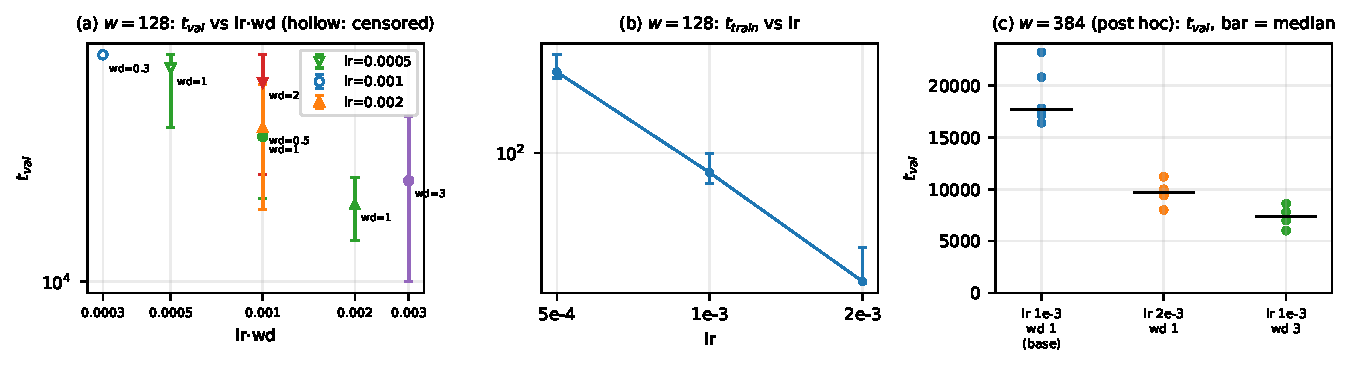
\includegraphics[width=\linewidth]{figs/fig_e4.pdf}
\caption{(a,b) MLP $w{=}128$, 7 (lr, wd) settings, 4 seeds each, $T_{max}=8\times10^4$: $\tva$ vs lr$\cdot$wd (median, bootstrap CI; marker = lr, colour = wd; (lr=$10^{-3}$, wd$=0.3$) censored in all runs) and $\ttr$ vs lr. (c) $w{=}384$, post-hoc test P8 (individual runs).}\label{fig:e4}
\end{figure}
P4 predicts that $\tva$ depends on lr and wd only via lr$\cdot$wd. At $w{=}128$ the log-log slope of $\tva$ on lr$\cdot$wd is $-0.62$ [$-0.83,-0.42$] (run-level bootstrap; 7/28 runs censored, which biases the slope towards 0), outside the registered $[-1.3,-0.7]$.
Three settings with identical product $10^{-3}$ (lr $5\!\times\!10^{-4},10^{-3},2\!\times\!10^{-3}$) give median $\tva$ of $62$k (1/4 censored), $37.8$k and $41.2$k: ratio $1.64>1.5$. A regression of $\log\tva$ on $\log$ lr and $\log$ wd gives exponents
$-0.82$ [$-1.09,-0.54$] for lr and $-0.55$ [$-0.78,-0.33$] for wd. \textbf{P4 is falsified} as registered at $w{=}128$. The memorisation clock is mostly an lr clock: $\ttr\propto \mathrm{lr}^{-0.77}$.

\emph{Post-hoc saturation test (P8).} Since $\tva$ flattens at large width, one expects it to be controlled by the optimiser at large width. At $w{=}384$ (4 seeds per setting; baseline 6 seeds), doubling lr reduces median $\tva$ from $17.7$k to $9.7$k (ratio $1.82$ [$1.58,2.39$]) and tripling wd to $7.4$k (ratio $2.39$ [$2.06,3.2$]): both exceed the registered factor 1.4 (\textbf{P8 supported}).
Together with P4: the generalisation clock follows lr$\cdot$wd approximately (exponents $\approx-0.8$) only at large width, while near the generalisation threshold it also depends on width.

\subsection{Robustness: tasks, modulus, parameterisation, architecture}\label{sec:robust}
\begin{figure}[t]
\centering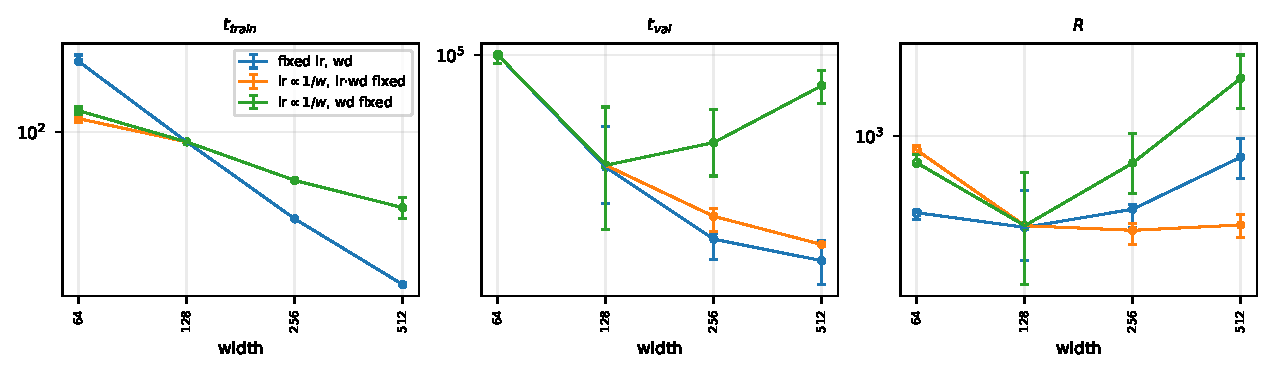
\includegraphics[width=\linewidth]{figs/fig_e7.pdf}
\caption{Width dependence under three scalings of lr/wd with width (MLP, $p{=}53$; reference $w{=}128$, lr $10^{-3}$, wd 1). Fixed lr, wd (6 seeds); lr$\propto1/w$ with lr$\cdot$wd fixed (4 seeds; 2 at $w{=}512$); lr$\propto1/w$ with wd fixed (same seeds). Hollow markers: censored.}\label{fig:e7}
\end{figure}
\textbf{Parameterisation (P7).} Fig.~\ref{fig:e7} and Table~\ref{tab:e7}: with lr$\propto1/w$ and lr$\cdot$wd fixed, the $\ttr$ slope for $w\ge128$ is $-0.50$ [$-0.58,-0.42$], the $\tva$ slope $-0.50$ [$-0.87,-0.09$], and the $R$ slope $+0.005$ [$-0.37,+0.42$]: $R$ is flat ($420,402,423$).
With lr$\propto1/w$ and wd fixed (decay rate $\propto1/w$), $\tva$ \emph{increases} with width (slope $+0.51$ [$+0.14,+0.92$]; $46$k at $w{=}256$, $76$k at $w{=}512$ with 2 seeds) and $R$ grows faster (slope $+1.03$ [$+0.57,+1.44$]).
Hence ``bigger models grok relatively later'' is parameterisation-dependent; the absolute generalisation time follows the decay rate (compare $\tva$ at $w{=}512$: $16.3$k fixed lr; $18.8$k fixed decay rate; $76$k decay rate $\propto1/w$). \textbf{P7 is supported.}
(The $w{=}128$ rows of the two scaled settings coincide because they are the same configuration run twice with identical seeds, which also confirms determinism.)

\begin{table}[t]\centering\scriptsize
\caption{Other operations and modulus (MLP, $f{=}0.3$, lr $10^{-3}$, wd 1). Median [95\% CI]; $\geq$: at least half of the runs censored at $10^5$ steps.}\label{tab:e6}
\begin{tabular}{llrcccc}
\toprule
task & $p$ & width & $t_{train}$ & $t_{val}$ & $R=t_{val}/t_{train}$ & cens./$n$ \\
\midrule
add & 53 & 64 & 210 & $\geq$100000 [100000,100000] & $\geq$476 & 6/6 \\
add & 53 & 128 & 90 & 37200 [26900,53200] & 413 & 0/6 \\
add & 53 & 256 & 40 & 19700 [16500,20700] & 492 & 0/6 \\
add & 97 & 64 & 470 & $\geq$100000 [100000,100000] & $\geq$213 & 3/3 \\
add & 97 & 128 & 160 & 54800 [51400,58200] & 342 & 0/3 \\
add & 97 & 256 & 70 & 13600 [12800,14400] & 194 & 0/3 \\
mul & 53 & 64 & 210 & $\geq$100000 [100000,100000] & $\geq$476 & 4/4 \\
mul & 53 & 128 & 90 & 39000 [28400,45800] & 433 & 0/4 \\
mul & 53 & 256 & 40 & 16500 [15600,18400] & 412 & 0/4 \\
sq & 53 & 64 & 200 & $\geq$83700 [66600,100000] & $\geq$407 & 2/4 \\
sq & 53 & 128 & 80 & $\geq$78300 [24200,100000] & $\geq$909 & 2/4 \\
sq & 53 & 256 & 40 & 25100 [17800,33200] & 628 & 0/4 \\
sub & 53 & 64 & 210 & $\geq$100000 [100000,100000] & $\geq$476 & 4/4 \\
sub & 53 & 128 & 90 & 30800 [29400,35800] & 342 & 0/4 \\
sub & 53 & 256 & 40 & 22000 [15600,24000] & 550 & 0/4 \\
\bottomrule
\end{tabular}
\end{table}
\textbf{Other operations and modulus (P5).} Table~\ref{tab:e6}: $\ttr$ falls with width in every task (P1 holds), and the absolute delay $D$ falls from $w{=}128$ to $256$ for all five tasks. The relative delay behaves differently across tasks:
$R$ rises from $128$ to $256$ for addition ($413\to492$) and subtraction ($342\to550$), is flat for multiplication ($433\to412$) and \emph{falls} for $p{=}97$ ($343\to194$); for $a^2{+}b^2$, $R$ at $w{=}128$ is a lower bound ($\ge909$, 2/4 censored), above $R$ at $w{=}256$ ($627$), so $R$ does not rise there either.
\textbf{P5 is therefore only partly supported}: P1 and the decrease of $D$ generalise; the increase of $R$ does not. For $p{=}97$, $w{=}64$ is censored for all 3 seeds, i.e.\ the generalisation threshold moves up with $p$.

\textbf{Transformer (P6).} One-layer transformer, $d_{model}\in\{16,32,64,128\}$ (5k--211k parameters), same optimiser, $T_{max}=4\times10^4$ steps ($10^5$ at $d_{model}{=}128$ after the first runs did not finish), 4 seeds (3 at $d_{model}{=}128$).
$\ttr$ falls monotonically ($1075,345,165,100$ steps; slope $-1.13$ [$-1.18,-1.08$]): P1 holds. For $d_{model}\le32$ validation accuracy stays below $0.09$ for all 8 runs within $4\times10^4$ steps; at $d_{model}{=}64$ three of four runs reach 99\% ($14$--$33$k steps);
at $d_{model}{=}128$ one of three reaches 99\% ($89$k) and the other two plateau at $0.97$--$0.98$ validation accuracy, so the 99\% criterion is brittle for this model; with a 95\% criterion (post hoc; Tab.~\ref{tab:e5}) all three reach it ($14.4$k, $27.4$k, $88$k).
The relative delay rises with width (median $R=180$ at $d_{model}{=}64$ with one censored run; $\ge890$ at 128 with 99\%), but the absolute delay does not fall: median $D=29.8$k at $64$ versus a lower bound of $99.9$k at 128 (99\%; 2/3 censored), and under 95\% the ranges overlap ($8.6$--$31.6$k vs $14.4$--$88$k).
So \textbf{P6 is partly supported} (P1 and the rise of $R$); the MLP behaviour of a falling $D$ is not reproduced, but our transformers are in the near-threshold regime ($d_{model}\le128$) where even MLPs show a steep $\tva(w)$, and the comparison has few seeds and a brittle criterion.

\begin{table}[t]\centering\small
\caption{Scorecard for registered predictions (details in the text).}\label{tab:score}
\begin{tabular}{p{3.5cm}p{4.6cm}p{4.8cm}}\toprule
Prediction & Verdict & Evidence \\\midrule
P1 $\ttr\downarrow$ in $w$ & supported & slope $-1.04$ to $-1.39$; all tasks \\
P2 $R\uparrow$, $D\not\uparrow$ & supported for add, $p{=}53$; not general & $R$ slope $+0.49$; fails $p{=}97$, mul \\
P3 label-agnostic fitting; threshold & partly: first half supported, second falsified at $f{=}0.5$ & $\rho{=}0.9999$; $16$ vs $32$ \\
P4 lr$\cdot$wd scaling ($w{=}128$) & falsified & slope $-0.62$; ratio $1.64$ \\
P5 other tasks/$p$ & partly & $D\downarrow$ everywhere; $R\uparrow$ only for add/sub \\
P6 transformer & partly: P1 and $R\uparrow$ supported; $D\downarrow$ not reproduced & slope $-1.13$; $D(128)\ge D(64)$; brittle 99\% criterion \\
P7 parameterisation & supported & $R$ slope $0.0$ vs $+1.0$ \\
P8 (post hoc) saturation & supported & lr$\times2$: $1.8\times$; wd$\times3$: $2.4\times$ \\\bottomrule
\end{tabular}
\end{table}

\section{Discussion and limitations}
\textbf{What the evidence supports.} In this controlled setting, width acts on grokking mainly by accelerating memorisation (a label-agnostic, lr-driven clock) much more than generalisation. Whether this makes
grokking ``more pronounced'' depends on the definition: relative delay rises in the core setting, absolute delay falls, and a narrow-model regime exists where generalisation needs about $10^3\times$ the steps of memorisation ($R\approx950$--$1300$ at $w{=}64$, $f{=}0.3$, two runs) or does not happen within the budget.
We did not find a width above which grokking disappears (largest $w{=}512$, 842k parameters; $R\approx800$). The negative results are informative for experimental design: (i) with fixed lr, wd, wider models reach generalisation sooner in absolute time but delay is not independent of how the optimiser is scaled;
(ii) a testbed that is ``too small'' will not show grokking within a typical budget; (iii) with more data some narrow models generalise directly.\\
\textbf{Relation to prior explanations.} The label-agnostic memorisation time and the importance of lr$\cdot$wd at large width agree with weight-decay-driven pictures~\citep{varma2023circuit,liu2023omnigrok}, and the parameterisation dependence is
what one would expect if width acts through the lazy/rich balance~\citep{kumar2024grokking}; we did not measure laziness or circuits, so these remain interpretations, not tests.\\
\textbf{Limitations.} (1) One small modulus ($p{=}53$; one check at $97$), one optimiser recipe (full-batch AdamW, $\beta_2{=}0.98$), and a single data fraction for most sweeps; minibatch noise, dropout and other regularisers were not studied.
(2) $\le6$ seeds per cell, so CIs are wide, and 3 seeds in the probes; seed variation of $\tva$ is large (e.g.\ $26.9$k--$53.2$k CI at $w{=}128$). (3) Censoring at $10^5$ steps (and $4\times10^5$ in one probe) means $\tva$ for narrow models is a bound, and the ``threshold'' depends on the budget. (4) $\ttr$ has a 10-step resolution, which matters for $w\ge256$ ($\ttr\le40$). (5) The two-clock account was refined after seeing the pilot and main sweeps; the confirmatory value is in the pre-registered predictions with fresh seeds (P1--P7), while P8 and the three-regime picture are post hoc.
(6) The transformer evidence is limited: $d_{model}\le128$, 3--4 seeds, a validation criterion that is brittle for this model (plateaus at $0.96$--$0.99$), and only the near-threshold regime. (7) Width above $512$ (MLP) and all depth effects were not studied; the MLP widths reach $842$k parameters, near the $10^6$ budget. (8) No mechanistic analysis. (9) Results are for a 99\% accuracy criterion.

\section{Conclusion}
On modular addition, model width speeds up memorisation roughly as $w^{-1}$ and generalisation more slowly, so grokking is relatively longer but absolutely shorter for wider MLPs at fixed lr and wd. This relative effect is not universal: it depends on the optimiser parameterisation, the modulus and the operation.
Narrow models that can fit the data still need orders of magnitude more steps to generalise (or do not within a practical budget), and with more data some of them skip the delay. We hope the scorecard against our self-registered predictions, including falsified predictions, helps calibrate future explanations of delayed generalisation.

\bibliographystyle{plainnat}
\bibliography{refs}

\appendix
\section{Reproduction map and compute}\label{app:exp}
\subsection*{A.1 Experiments, scripts and artefacts}
All code is in \texttt{code/}; \texttt{code/README.md} gives the commands. Each experiment is a function in \texttt{code/experiments.py}, run with \texttt{python sweep.py <name> <n\_procs>}, which appends one JSON line per run (including the full accuracy/loss/parameter-norm curve) to \texttt{results/<name>.jsonl}.
\texttt{python analysis.py} regenerates every figure (\texttt{paper/figs}), table (\texttt{paper/tables}) and number quoted in the text (\texttt{results/summary.json}).
\begin{center}\scriptsize
\begin{tabular}{p{2.3cm}p{5.8cm}p{1.1cm}p{3.2cm}}\toprule
Experiment & Configuration (seeds) & Runs & Used for\\\midrule
\texttt{e1\_mlp\_width} & MLP, $p{=}53$, add, $f{=}0.3$, $w\in\{24,\dots,512\}$ (10 widths), $T_{max}{=}10^5$ (100--105) & 60 & Fig.~\ref{fig:e1}, Tab.~\ref{tab:e1}, Fig.~\ref{fig:probe}c, \ref{fig:thresh}\\
\texttt{e2\_random} & as e1, random train labels (100--102) & 30 & Fig.~\ref{fig:probe}\\
\texttt{e3\_frac} & $f\in\{0.2,0.5\}$, $w\in\{24..256\}$, real (100--102) and random labels (100--102), $T_{max}{=}6\!\times\!10^4$ & 96 & Fig.~\ref{fig:probe}, \ref{fig:thresh}, \ref{fig:frac}\\
\texttt{e8\_small} & $w\in\{8,12,16,20\}$, $f\in\{0.2,0.3,0.5\}$, real and random labels (100--103), $T_{max}{=}6\!\times\!10^4$ (added after seeing that e2 fits from $w{=}24$) & 96 & Fig.~\ref{fig:probe}, \ref{fig:thresh}\\
\texttt{e10\_threshold} & $w\in\{72,80,88\}$, $f{=}0.3$ (100--105), $10^5$ steps (post hoc) & 18 & Sec.~\ref{sec:thresh}\\
\texttt{e9\_long} & $w\in\{48,64\}$, $f{=}0.3$, $T_{max}{=}4\!\times\!10^5$ (100--102) (post hoc) & 6 & Fig.~\ref{fig:thresh}\\
\texttt{e4\_timescale} & $w{=}128$; 7 (lr,wd) pairs; $T_{max}{=}8\!\times\!10^4$ (100--103) & 28 & Fig.~\ref{fig:e4}\\
\texttt{e11\_saturation} & $w{=}384$; (lr,wd)$\in\{(2\!\times\!10^{-3},1),(10^{-3},3)\}$; $T_{max}{=}6\!\times\!10^4$ (100--103) (post hoc, P8) & 8 & Sec.~\ref{sec:timescale}\\
\texttt{e6\_generality} & sub, mul, $a^2{+}b^2$ ($p{=}53$) and add ($p{=}97$), $w\in\{64,128,256\}$ (100--103; 100--102 for $p{=}97$) & 45 & Tab.~\ref{tab:e6}, Fig.~\ref{fig:e6}\\
\texttt{e7\_param} & lr$\propto1/w$, wd$\propto w$ or fixed; $w\in\{64..512\}$ (100--103; 100--101 at $w{=}512$) & 28 & Fig.~\ref{fig:e7}, Tab.~\ref{tab:e7}\\
\texttt{e5\_tf}, \texttt{e5b\_tf\_small}, \texttt{e12\_tf128\_long} & transformer, $d_{model}\in\{16,32,64,128\}$, $p{=}53$, $T_{max}{=}4\!\times\!10^4$ (100--103); $d_{model}{=}128$ re-run with $T_{max}{=}10^5$ (100--102, post hoc) & 16 + 3 & Sec.~\ref{sec:robust}, Fig.~\ref{fig:e5}, Tab.~\ref{tab:e5}\\
\texttt{pilot}, \texttt{pilot\_mlp} & exploratory pilot (seeds 0--2, 30k steps); both aborted when the compute budget was re-planned (partial) & 17 & motivates hypotheses only; not used in any reported statistic\\\bottomrule
\end{tabular}
\end{center}

\subsection*{A.2 Additional tables and figures}
\begin{table}[h]\centering\scriptsize
\caption{Width-scaling variants (Fig.~\ref{fig:e7}). The two scaled settings coincide at the reference width $w{=}128$ (same configuration and seeds).}\label{tab:e7}
\begin{tabular}{llrcccc}
\toprule
setting & width & lr & $t_{train}$ & $t_{val}$ & $R$ & cens./$n$ \\
\midrule
fixed lr, wd & 64 & 0.001 & 210 & $\geq$100000 [100000,100000] & $\geq$476 & 6/6 \\
fixed lr, wd & 128 & 0.001 & 90 & 37200 [26900,53200] & 413 & 0/6 \\
fixed lr, wd & 256 & 0.001 & 40 & 19700 [16500,20700] & 492 & 0/6 \\
fixed lr, wd & 512 & 0.001 & 20 & 16300 [13200,19500] & 815 & 0/6 \\
lr$\propto1/w$, lr$\cdot$wd fixed & 64 & 0.002 & 115 & $\geq$100000 [100000,100000] & $\geq$871 & 4/4 \\
lr$\propto1/w$, lr$\cdot$wd fixed & 128 & 0.001 & 90 & 37800 [21400,63200] & 420 & 0/4 \\
lr$\propto1/w$, lr$\cdot$wd fixed & 256 & 0.0005 & 60 & 24100 [21000,25800] & 402 & 0/4 \\
lr$\propto1/w$, lr$\cdot$wd fixed & 512 & 0.00025 & 45 & 18800 [18800,18800] & 423 & 0/2 \\
lr$\propto1/w$, wd fixed & 64 & 0.002 & 125 & $\geq$100000 [92800,100000] & $\geq$771 & 3/4 \\
lr$\propto1/w$, wd fixed & 128 & 0.001 & 90 & 37800 [21400,63200] & 420 & 0/4 \\
lr$\propto1/w$, wd fixed & 256 & 0.0005 & 60 & 46200 [34400,61600] & 770 & 0/4 \\
lr$\propto1/w$, wd fixed & 512 & 0.00025 & 45 & 76300 [65200,87400] & 1744 & 0/2 \\
\bottomrule
\end{tabular}
\end{table}
\begin{figure}[h]\centering
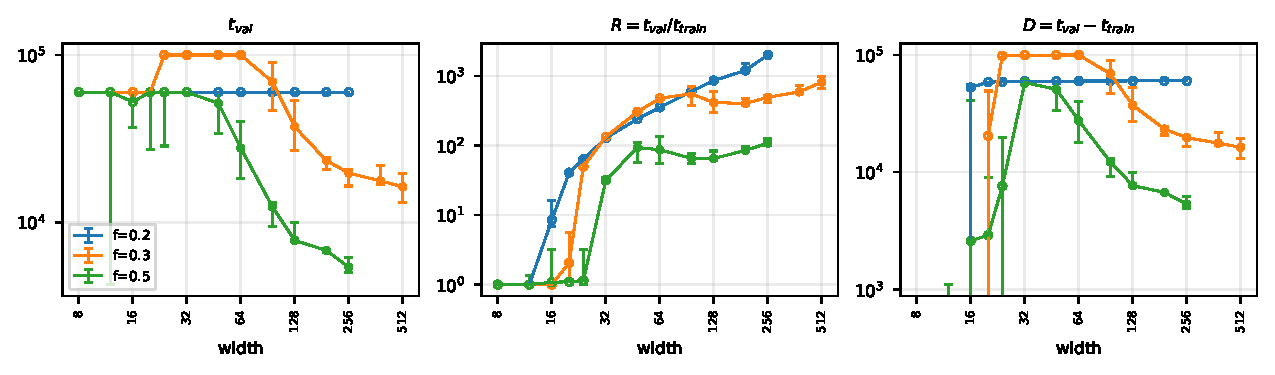
\includegraphics[width=.9\linewidth]{figs/fig_frac.pdf}
\caption{$t_{val}$, $R$, $D$ vs.\ width for three training fractions (MLP, $p{=}53$; $10^5$ steps for $f{=}0.3$, $6\!\times\!10^4$ for $f{=}0.2,0.5$; hollow: mostly censored). Only the $f{=}0.3$ line extends beyond $w{=}256$.}\label{fig:frac}
\end{figure}
\begin{figure}[h]\centering
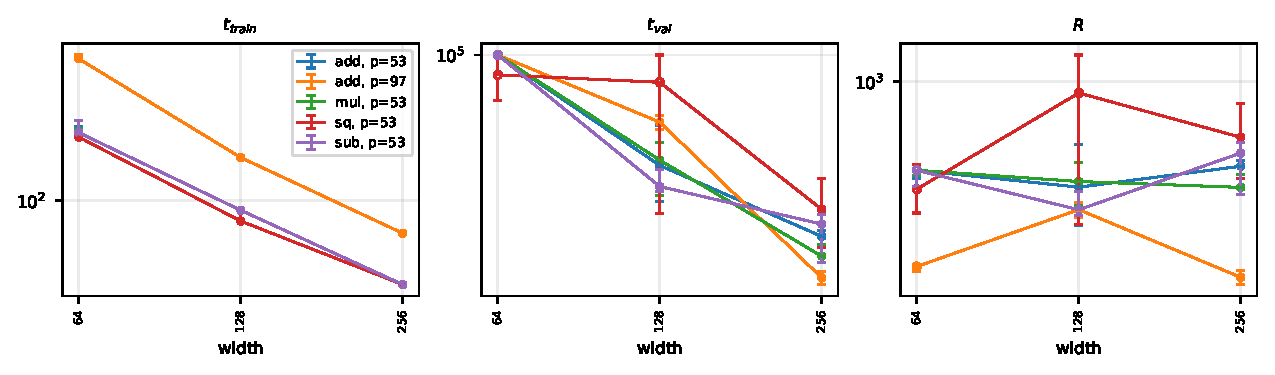
\includegraphics[width=.9\linewidth]{figs/fig_e6.pdf}
\caption{Other operations and modulus (Tab.~\ref{tab:e6}).}\label{fig:e6}
\end{figure}
\begin{table}[h]\centering\scriptsize
\caption{Transformer runs (seeds 100--103; 100--102 at $d_{model}{=}128$). Per-seed times to 99\% and (post hoc) 95\% validation accuracy; $-$: not reached within the budget. Max.\ val.\ acc.: highest validation accuracy over the run.}\label{tab:e5}
\begin{tabular}{rrrcccc}
\toprule
$d_{model}$ & params & budget & $t_{train}$ & $t_{val}$, 99\% (per seed) & $t_{val}$, 95\% (per seed) & max val.\ acc.\ \\
\midrule
16 & 5k & 40k & 1075 & $-$, $-$, $-$, $-$ & $-$, $-$, $-$, $-$ & 0.04, 0.02, 0.08, 0.04 \\
32 & 16k & 40k & 345 & $-$, $-$, $-$, $-$ & $-$, $-$, $-$, $-$ & 0.02, 0.07, 0.03, 0.02 \\
64 & 57k & 40k & 165 & $-$, 26.2k, 14.2k, 33.4k & $-$, 19.8k, 8.6k, 31.6k & 0.03, 0.99, 0.99, 0.99 \\
128 & 211k & 100k & 100 & $-$, 89.0k, $-$ & 27.4k, 88.0k, 14.4k & 0.99, 0.99, 0.99 \\
\bottomrule
\end{tabular}
\end{table}
\begin{figure}[h]\centering
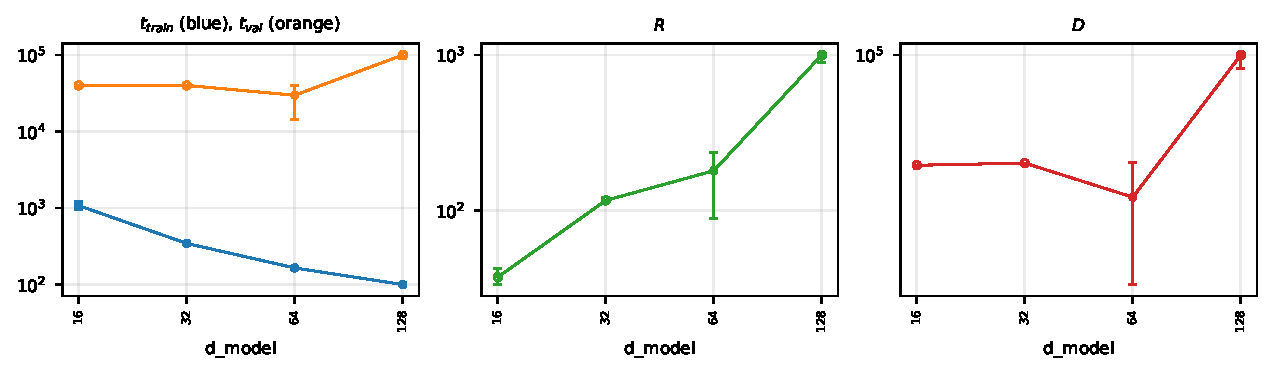
\includegraphics[width=.9\linewidth]{figs/fig_e5.pdf}
\caption{Transformer: $t_{train}$ and $t_{val}$ (99\%), $R$, $D$ vs $d_{model}$ (medians, bootstrap CIs; hollow: mostly censored).}\label{fig:e5}
\end{figure}

\subsection*{A.3 Environment, seeds, cost}
Python 3.11.15, PyTorch 2.15.0+cpu (CPU only, 1 thread per run), NumPy 2.4.6, SciPy 1.17.1, Matplotlib 3.11.2; LaTeX: TeX Live \texttt{pdflatex}/\texttt{latexmk}. Seeds: 0--2 (pilot), 100+ (all reported experiments); the seed sets both model initialisation and the train/validation split (split seed $=10000+$seed). Runs are deterministic for a given (config, seed) on a given machine (verified: duplicate configurations in e7 gave identical results).
The sandbox provided about 4--5 effective CPU cores shared with other tenants; the per-run wall-clock seconds in \texttt{results/*.jsonl} include contention. Summed per-run wall-clock time over all stored runs is given by \texttt{python code/compute\_stats.py} (\texttt{code/logs/compute\_stats.log}); it is 78 hours over all stored runs (434 reported runs plus 12 duplicated transformer runs and 17 pilot runs), most of it contention-inflated; the whole project took roughly 11 hours of wall-clock on this shared slice.

\subsection*{A.4 Deviations, failed or abandoned runs, and honest notes}
\begin{itemize}\setlength\itemsep{0pt}
\item \textbf{Template.} The official NeurIPS 2025 style file (the newest we could obtain: the 2026 archive was not available at the expected URL) is used in \texttt{preprint} mode (non-anonymous author line), with the NeurIPS checklist included.
\item \textbf{Compute-driven choices.} $p{=}53$ rather than $97$ (the latter is $\approx3\times$ costlier; checked only for 3 widths); transformer limited to $d_{model}\le128$ and $4\times10^4$ steps. An exploratory transformer pilot with $d_{model}$ up to 256 and an MLP pilot with $w\in\{512,1024\}$ were stopped for cost; their partial output is in \texttt{results/pilot*.jsonl} and is not used.
\item \textbf{Registration timing.} \texttt{PREREG.md} was written before e1 and e2 were launched. It is a self-registered file in the workspace (not an external registry), and the results of e2 (including the near-identical memorisation times) were visible before e3--e7 were launched; no prediction was changed afterwards, but P3's second half and the choice of e3/e4 grids could in principle have been influenced by e2.
\item \textbf{Post-hoc additions} (marked in the text): e8, e9, e10, e11, the three-regime interpretation, the saturation reading, and the choice to report $p{=}97$ for only 3 widths. The registered predictions P1--P7 were not edited after the sweeps (the file \texttt{code/PREREG.md} has an explicit addendum for P8).
\item \textbf{Analysis changes after seeing data.} The slope for $\ttr$ and $\tva$ is reported over fully-fitting/uncensored widths because including censored widths mixes bounds with values; the all-width slope for $\ttr$ is also given. The e4 regression treats censored runs as bounds (biased toward flatter slopes), a censoring-aware estimator (Tobit or survival regression) was not implemented. For the transformer, the 95\% validation criterion was added after observing plateaus just below 99\%.
\item \textbf{Parallel duplicates.} Because of a restart, some transformer configurations were queued twice; duplicate keys are dropped when loading (first result kept).
\item \textbf{Literature.} References were checked to exist via their arXiv abstract pages (\texttt{code/check\_refs.py}, \texttt{code/logs/refs\_check.log}); statements about their content in Sec.~2 follow the one-line descriptions in the task's starter list and our prior knowledge; the full texts were not re-read during this run. No other literature search was run.
\item \textbf{LLM usage.} The research design, code, experiments, analysis and this manuscript were produced by an autonomous LLM-based agent running unattended; no human reviewed the intermediate results. The studied models are small MLPs and transformers trained from scratch; no LLM is part of the experimental pipeline.
\item \textbf{Restricted content.} No search for, access to, or reading of the restricted paper(s) described in the task brief was performed; no web pages other than the NeurIPS style-file archive, pip packages and the arXiv abstract pages listed above were accessed. Nothing restricted was encountered.
\end{itemize}


\newpage
\newpage
\section*{NeurIPS Paper Checklist}




\begin{enumerate}

\item {\bf Claims}
    \item[] Question: Do the main claims made in the abstract and introduction accurately reflect the paper's contributions and scope?
    \item[] Answer: \answerYes{} % Replace by \answerYes{}, \answerNo{}, or \answerNA{}.
    \item[] Justification: The abstract and Sec.~1 state the measured relations (with CIs) and the falsified predictions; scope limits ($p{=}53$, one optimiser recipe, $\le6$ seeds) are stated in the abstract and Sec.~5.
    \item[] Guidelines:
    \begin{itemize}
        \item The answer NA means that the abstract and introduction do not include the claims made in the paper.
        \item The abstract and/or introduction should clearly state the claims made, including the contributions made in the paper and important assumptions and limitations. A No or NA answer to this question will not be perceived well by the reviewers. 
        \item The claims made should match theoretical and experimental results, and reflect how much the results can be expected to generalize to other settings. 
        \item It is fine to include aspirational goals as motivation as long as it is clear that these goals are not attained by the paper. 
    \end{itemize}

\item {\bf Limitations}
    \item[] Question: Does the paper discuss the limitations of the work performed by the authors?
    \item[] Answer: \answerYes{} % Replace by \answerYes{}, \answerNo{}, or \answerNA{}.
    \item[] Justification: Sec.~5 (Discussion and limitations) lists nine limitations (modulus, recipe, seeds, censoring, resolution, post-hoc analyses, transformer evidence, scale range, no mechanistic analysis).
    \item[] Guidelines:
    \begin{itemize}
        \item The answer NA means that the paper has no limitation while the answer No means that the paper has limitations, but those are not discussed in the paper. 
        \item The authors are encouraged to create a separate "Limitations" section in their paper.
        \item The paper should point out any strong assumptions and how robust the results are to violations of these assumptions (e.g., independence assumptions, noiseless settings, model well-specification, asymptotic approximations only holding locally). The authors should reflect on how these assumptions might be violated in practice and what the implications would be.
        \item The authors should reflect on the scope of the claims made, e.g., if the approach was only tested on a few datasets or with a few runs. In general, empirical results often depend on implicit assumptions, which should be articulated.
        \item The authors should reflect on the factors that influence the performance of the approach. For example, a facial recognition algorithm may perform poorly when image resolution is low or images are taken in low lighting. Or a speech-to-text system might not be used reliably to provide closed captions for online lectures because it fails to handle technical jargon.
        \item The authors should discuss the computational efficiency of the proposed algorithms and how they scale with dataset size.
        \item If applicable, the authors should discuss possible limitations of their approach to address problems of privacy and fairness.
        \item While the authors might fear that complete honesty about limitations might be used by reviewers as grounds for rejection, a worse outcome might be that reviewers discover limitations that aren't acknowledged in the paper. The authors should use their best judgment and recognize that individual actions in favor of transparency play an important role in developing norms that preserve the integrity of the community. Reviewers will be specifically instructed to not penalize honesty concerning limitations.
    \end{itemize}

\item {\bf Theory assumptions and proofs}
    \item[] Question: For each theoretical result, does the paper provide the full set of assumptions and a complete (and correct) proof?
    \item[] Answer: \answerNA{} % Replace by \answerYes{}, \answerNo{}, or \answerNA{}.
    \item[] Justification: The paper contains no theoretical results.
    \item[] Guidelines:
    \begin{itemize}
        \item The answer NA means that the paper does not include theoretical results. 
        \item All the theorems, formulas, and proofs in the paper should be numbered and cross-referenced.
        \item All assumptions should be clearly stated or referenced in the statement of any theorems.
        \item The proofs can either appear in the main paper or the supplemental material, but if they appear in the supplemental material, the authors are encouraged to provide a short proof sketch to provide intuition. 
        \item Inversely, any informal proof provided in the core of the paper should be complemented by formal proofs provided in appendix or supplemental material.
        \item Theorems and Lemmas that the proof relies upon should be properly referenced. 
    \end{itemize}

    \item {\bf Experimental result reproducibility}
    \item[] Question: Does the paper fully disclose all the information needed to reproduce the main experimental results of the paper to the extent that it affects the main claims and/or conclusions of the paper (regardless of whether the code and data are provided or not)?
    \item[] Answer: \answerYes{} % Replace by \answerYes{}, \answerNo{}, or \answerNA{}.
    \item[] Justification: Sec.~3 and App.~A give data generation, architectures, optimiser, metrics, seeds and the statistics; code regenerates every number.
    \item[] Guidelines:
    \begin{itemize}
        \item The answer NA means that the paper does not include experiments.
        \item If the paper includes experiments, a No answer to this question will not be perceived well by the reviewers: Making the paper reproducible is important, regardless of whether the code and data are provided or not.
        \item If the contribution is a dataset and/or model, the authors should describe the steps taken to make their results reproducible or verifiable. 
        \item Depending on the contribution, reproducibility can be accomplished in various ways. For example, if the contribution is a novel architecture, describing the architecture fully might suffice, or if the contribution is a specific model and empirical evaluation, it may be necessary to either make it possible for others to replicate the model with the same dataset, or provide access to the model. In general. releasing code and data is often one good way to accomplish this, but reproducibility can also be provided via detailed instructions for how to replicate the results, access to a hosted model (e.g., in the case of a large language model), releasing of a model checkpoint, or other means that are appropriate to the research performed.
        \item While NeurIPS does not require releasing code, the conference does require all submissions to provide some reasonable avenue for reproducibility, which may depend on the nature of the contribution. For example
        \begin{enumerate}
            \item If the contribution is primarily a new algorithm, the paper should make it clear how to reproduce that algorithm.
            \item If the contribution is primarily a new model architecture, the paper should describe the architecture clearly and fully.
            \item If the contribution is a new model (e.g., a large language model), then there should either be a way to access this model for reproducing the results or a way to reproduce the model (e.g., with an open-source dataset or instructions for how to construct the dataset).
            \item We recognize that reproducibility may be tricky in some cases, in which case authors are welcome to describe the particular way they provide for reproducibility. In the case of closed-source models, it may be that access to the model is limited in some way (e.g., to registered users), but it should be possible for other researchers to have some path to reproducing or verifying the results.
        \end{enumerate}
    \end{itemize}


\item {\bf Open access to data and code}
    \item[] Question: Does the paper provide open access to the data and code, with sufficient instructions to faithfully reproduce the main experimental results, as described in supplemental material?
    \item[] Answer: \answerYes{} % Replace by \answerYes{}, \answerNo{}, or \answerNA{}.
    \item[] Justification: All code is in the supplementary \texttt{code/} directory with a README listing environment versions, exact commands and run times; data are synthetic and generated in memory.
    \item[] Guidelines:
    \begin{itemize}
        \item The answer NA means that paper does not include experiments requiring code.
        \item Please see the NeurIPS code and data submission guidelines (\url{https://nips.cc/public/guides/CodeSubmissionPolicy}) for more details.
        \item While we encourage the release of code and data, we understand that this might not be possible, so “No” is an acceptable answer. Papers cannot be rejected simply for not including code, unless this is central to the contribution (e.g., for a new open-source benchmark).
        \item The instructions should contain the exact command and environment needed to run to reproduce the results. See the NeurIPS code and data submission guidelines (\url{https://nips.cc/public/guides/CodeSubmissionPolicy}) for more details.
        \item The authors should provide instructions on data access and preparation, including how to access the raw data, preprocessed data, intermediate data, and generated data, etc.
        \item The authors should provide scripts to reproduce all experimental results for the new proposed method and baselines. If only a subset of experiments are reproducible, they should state which ones are omitted from the script and why.
        \item At submission time, to preserve anonymity, the authors should release anonymized versions (if applicable).
        \item Providing as much information as possible in supplemental material (appended to the paper) is recommended, but including URLs to data and code is permitted.
    \end{itemize}


\item {\bf Experimental setting/details}
    \item[] Question: Does the paper specify all the training and test details (e.g., data splits, hyperparameters, how they were chosen, type of optimizer, etc.) necessary to understand the results?
    \item[] Answer: \answerYes{} % Replace by \answerYes{}, \answerNo{}, or \answerNA{}.
    \item[] Justification: Sec.~3 and App.~A: architectures, initialisation, optimiser settings, evaluation schedule, splits and seeds; hyperparameters were fixed a priori (they follow common grokking setups) and varied only in the reported sweeps.
    \item[] Guidelines:
    \begin{itemize}
        \item The answer NA means that the paper does not include experiments.
        \item The experimental setting should be presented in the core of the paper to a level of detail that is necessary to appreciate the results and make sense of them.
        \item The full details can be provided either with the code, in appendix, or as supplemental material.
    \end{itemize}

\item {\bf Experiment statistical significance}
    \item[] Question: Does the paper report error bars suitably and correctly defined or other appropriate information about the statistical significance of the experiments?
    \item[] Answer: \answerYes{} % Replace by \answerYes{}, \answerNo{}, or \answerNA{}.
    \item[] Justification: Medians with 95\% bootstrap CIs over seeds (seed = initialisation and data split) in all figures/tables; log-log slopes and Spearman correlations have bootstrap CIs; censoring is handled as lower bounds. $n\le6$ so CIs are coarse; no multiple-testing correction (stated in Sec.~4).
    \item[] Guidelines:
    \begin{itemize}
        \item The answer NA means that the paper does not include experiments.
        \item The authors should answer "Yes" if the results are accompanied by error bars, confidence intervals, or statistical significance tests, at least for the experiments that support the main claims of the paper.
        \item The factors of variability that the error bars are capturing should be clearly stated (for example, train/test split, initialization, random drawing of some parameter, or overall run with given experimental conditions).
        \item The method for calculating the error bars should be explained (closed form formula, call to a library function, bootstrap, etc.)
        \item The assumptions made should be given (e.g., Normally distributed errors).
        \item It should be clear whether the error bar is the standard deviation or the standard error of the mean.
        \item It is OK to report 1-sigma error bars, but one should state it. The authors should preferably report a 2-sigma error bar than state that they have a 96\% CI, if the hypothesis of Normality of errors is not verified.
        \item For asymmetric distributions, the authors should be careful not to show in tables or figures symmetric error bars that would yield results that are out of range (e.g. negative error rates).
        \item If error bars are reported in tables or plots, The authors should explain in the text how they were calculated and reference the corresponding figures or tables in the text.
    \end{itemize}

\item {\bf Experiments compute resources}
    \item[] Question: For each experiment, does the paper provide sufficient information on the computer resources (type of compute workers, memory, time of execution) needed to reproduce the experiments?
    \item[] Answer: \answerYes{} % Replace by \answerYes{}, \answerNo{}, or \answerNA{}.
    \item[] Justification: App.~A.3: CPU only (about 4--5 effective shared cores), per-run wall-clock recorded in the results files, about 65 summed run-hours; pilot and aborted runs are disclosed.
    \item[] Guidelines:
    \begin{itemize}
        \item The answer NA means that the paper does not include experiments.
        \item The paper should indicate the type of compute workers CPU or GPU, internal cluster, or cloud provider, including relevant memory and storage.
        \item The paper should provide the amount of compute required for each of the individual experimental runs as well as estimate the total compute. 
        \item The paper should disclose whether the full research project required more compute than the experiments reported in the paper (e.g., preliminary or failed experiments that didn't make it into the paper). 
    \end{itemize}
    
\item {\bf Code of ethics}
    \item[] Question: Does the research conducted in the paper conform, in every respect, with the NeurIPS Code of Ethics \url{https://neurips.cc/public/EthicsGuidelines}?
    \item[] Answer: \answerYes{} % Replace by \answerYes{}, \answerNo{}, or \answerNA{}.
    \item[] Justification: The work uses only synthetic data, no human subjects, and follows the Code of Ethics as far as we can assess.
    \item[] Guidelines:
    \begin{itemize}
        \item The answer NA means that the authors have not reviewed the NeurIPS Code of Ethics.
        \item If the authors answer No, they should explain the special circumstances that require a deviation from the Code of Ethics.
        \item The authors should make sure to preserve anonymity (e.g., if there is a special consideration due to laws or regulations in their jurisdiction).
    \end{itemize}


\item {\bf Broader impacts}
    \item[] Question: Does the paper discuss both potential positive societal impacts and negative societal impacts of the work performed?
    \item[] Answer: \answerNA{} % Replace by \answerYes{}, \answerNo{}, or \answerNA{}.
    \item[] Justification: Foundational study of small synthetic tasks; we see no direct societal impact beyond general ML understanding.
    \item[] Guidelines:
    \begin{itemize}
        \item The answer NA means that there is no societal impact of the work performed.
        \item If the authors answer NA or No, they should explain why their work has no societal impact or why the paper does not address societal impact.
        \item Examples of negative societal impacts include potential malicious or unintended uses (e.g., disinformation, generating fake profiles, surveillance), fairness considerations (e.g., deployment of technologies that could make decisions that unfairly impact specific groups), privacy considerations, and security considerations.
        \item The conference expects that many papers will be foundational research and not tied to particular applications, let alone deployments. However, if there is a direct path to any negative applications, the authors should point it out. For example, it is legitimate to point out that an improvement in the quality of generative models could be used to generate deepfakes for disinformation. On the other hand, it is not needed to point out that a generic algorithm for optimizing neural networks could enable people to train models that generate Deepfakes faster.
        \item The authors should consider possible harms that could arise when the technology is being used as intended and functioning correctly, harms that could arise when the technology is being used as intended but gives incorrect results, and harms following from (intentional or unintentional) misuse of the technology.
        \item If there are negative societal impacts, the authors could also discuss possible mitigation strategies (e.g., gated release of models, providing defenses in addition to attacks, mechanisms for monitoring misuse, mechanisms to monitor how a system learns from feedback over time, improving the efficiency and accessibility of ML).
    \end{itemize}
    
\item {\bf Safeguards}
    \item[] Question: Does the paper describe safeguards that have been put in place for responsible release of data or models that have a high risk for misuse (e.g., pretrained language models, image generators, or scraped datasets)?
    \item[] Answer: \answerNA{} % Replace by \answerYes{}, \answerNo{}, or \answerNA{}.
    \item[] Justification: No models or data with misuse risk are released.
    \item[] Guidelines:
    \begin{itemize}
        \item The answer NA means that the paper poses no such risks.
        \item Released models that have a high risk for misuse or dual-use should be released with necessary safeguards to allow for controlled use of the model, for example by requiring that users adhere to usage guidelines or restrictions to access the model or implementing safety filters. 
        \item Datasets that have been scraped from the Internet could pose safety risks. The authors should describe how they avoided releasing unsafe images.
        \item We recognize that providing effective safeguards is challenging, and many papers do not require this, but we encourage authors to take this into account and make a best faith effort.
    \end{itemize}

\item {\bf Licenses for existing assets}
    \item[] Question: Are the creators or original owners of assets (e.g., code, data, models), used in the paper, properly credited and are the license and terms of use explicitly mentioned and properly respected?
    \item[] Answer: \answerYes{} % Replace by \answerYes{}, \answerNo{}, or \answerNA{}.
    \item[] Justification: Only open-source libraries (PyTorch, NumPy, SciPy, Matplotlib) and the NeurIPS style files are used, cited in App.~A.3; no third-party data.
    \item[] Guidelines:
    \begin{itemize}
        \item The answer NA means that the paper does not use existing assets.
        \item The authors should cite the original paper that produced the code package or dataset.
        \item The authors should state which version of the asset is used and, if possible, include a URL.
        \item The name of the license (e.g., CC-BY 4.0) should be included for each asset.
        \item For scraped data from a particular source (e.g., website), the copyright and terms of service of that source should be provided.
        \item If assets are released, the license, copyright information, and terms of use in the package should be provided. For popular datasets, \url{paperswithcode.com/datasets} has curated licenses for some datasets. Their licensing guide can help determine the license of a dataset.
        \item For existing datasets that are re-packaged, both the original license and the license of the derived asset (if it has changed) should be provided.
        \item If this information is not available online, the authors are encouraged to reach out to the asset's creators.
    \end{itemize}

\item {\bf New assets}
    \item[] Question: Are new assets introduced in the paper well documented and is the documentation provided alongside the assets?
    \item[] Answer: \answerYes{} % Replace by \answerYes{}, \answerNo{}, or \answerNA{}.
    \item[] Justification: The new code and result files are documented in \texttt{code/README.md}; no new datasets (data are generated by a few lines of code).
    \item[] Guidelines:
    \begin{itemize}
        \item The answer NA means that the paper does not release new assets.
        \item Researchers should communicate the details of the dataset/code/model as part of their submissions via structured templates. This includes details about training, license, limitations, etc. 
        \item The paper should discuss whether and how consent was obtained from people whose asset is used.
        \item At submission time, remember to anonymize your assets (if applicable). You can either create an anonymized URL or include an anonymized zip file.
    \end{itemize}

\item {\bf Crowdsourcing and research with human subjects}
    \item[] Question: For crowdsourcing experiments and research with human subjects, does the paper include the full text of instructions given to participants and screenshots, if applicable, as well as details about compensation (if any)? 
    \item[] Answer: \answerNA{} % Replace by \answerYes{}, \answerNo{}, or \answerNA{}.
    \item[] Justification: No crowdsourcing or human subjects.
    \item[] Guidelines:
    \begin{itemize}
        \item The answer NA means that the paper does not involve crowdsourcing nor research with human subjects.
        \item Including this information in the supplemental material is fine, but if the main contribution of the paper involves human subjects, then as much detail as possible should be included in the main paper. 
        \item According to the NeurIPS Code of Ethics, workers involved in data collection, curation, or other labor should be paid at least the minimum wage in the country of the data collector. 
    \end{itemize}

\item {\bf Institutional review board (IRB) approvals or equivalent for research with human subjects}
    \item[] Question: Does the paper describe potential risks incurred by study participants, whether such risks were disclosed to the subjects, and whether Institutional Review Board (IRB) approvals (or an equivalent approval/review based on the requirements of your country or institution) were obtained?
    \item[] Answer: \answerNA{} % Replace by \answerYes{}, \answerNo{}, or \answerNA{}.
    \item[] Justification: No human subjects.
    \item[] Guidelines:
    \begin{itemize}
        \item The answer NA means that the paper does not involve crowdsourcing nor research with human subjects.
        \item Depending on the country in which research is conducted, IRB approval (or equivalent) may be required for any human subjects research. If you obtained IRB approval, you should clearly state this in the paper. 
        \item We recognize that the procedures for this may vary significantly between institutions and locations, and we expect authors to adhere to the NeurIPS Code of Ethics and the guidelines for their institution. 
        \item For initial submissions, do not include any information that would break anonymity (if applicable), such as the institution conducting the review.
    \end{itemize}

\item {\bf Declaration of LLM usage}
    \item[] Question: Does the paper describe the usage of LLMs if it is an important, original, or non-standard component of the core methods in this research? Note that if the LLM is used only for writing, editing, or formatting purposes and does not impact the core methodology, scientific rigorousness, or originality of the research, declaration is not required.
    %this research? 
    \item[] Answer: \answerYes{} % Replace by \answerYes{}, \answerNo{}, or \answerNA{}.
    \item[] Justification: The research was conceived, run, analysed and written by an autonomous LLM-based research agent (no human in the loop during the run); this is declared in App.~A.4. LLMs are not part of the studied models.
    \item[] Guidelines:
    \begin{itemize}
        \item The answer NA means that the core method development in this research does not involve LLMs as any important, original, or non-standard components.
        \item Please refer to our LLM policy (\url{https://neurips.cc/Conferences/2025/LLM}) for what should or should not be described.
    \end{itemize}

\end{enumerate}

\end{document}
